%\documentclass[aps,prl,twocolumn,nobibnotes]{revtex4}
\documentclass[aps,twocolumn,nobibnotes]{revtex4}
%\documentclass[aps,preprint,showpacs,nobibnotes]{revtex4}
%\documentclass[aps,preprint,nobibnotes]{revtex}
\usepackage{graphics,graphicx,amsfonts,amsmath,amsbsy,amssymb,color}
\usepackage{bm}
\usepackage[a4paper,vmargin={20mm,20mm},hmargin={20mm,10mm}]{geometry}
%\usepackage{epic}
%\usepackage{mciteplus}
\usepackage{subfigure}
\usepackage{paralist}
\usepackage{vector}  % Allows "\bvec{}" and "\buvec{}" for "blackboard" style bold vectors in maths
\newcommand{\D}[1] {D_{\bf #1}}
\def \beq {\begin{eqnarray}}
\def \eeq {\end{eqnarray}}
\def \Schrodinger {{Schr\"{o}dinger }}
\def \Di {{D_{\bfi}}}
\def \Dj {{D_{\bfj}}}
\newcommand {\adag}[1] {{a_{#1}^\dagger}}
\def \bfj {{\bf j}}
\def \bfi {{\bf i}}
\def \rone {{\bvec{r}_1}}
\def \rtwo {{\bvec{r}_2}}
\def \mEh {{\textrm{mE}_{\textrm{h}}}}
\def \Eh {{\textrm{E}_{\textrm{h}}}}
\def \nadd {{n_a}}
\newcommand{\braket}[3] {{\langle #1 | #2 | #3 \rangle}}
\newcommand{\brket}[2] {{\langle #1 | #2 \rangle}}
\newcommand{\bra}{\ensuremath{\langle}}
\newcommand{\ket}{\ensuremath{\rangle}}
%\def \ham {{\bf H}}
\def \ham {{\hat{H}}}
%\def \Sz {{\hat{\textrm{S}_{\textrm{z}}}}}
\def \Sz {{\hat{S}_z}}
\newcommand{\rff}[1]{{Eq.~\eqref{#1}}}
\def \Pgen {{P_{\textrm{gen}}}}
\def \Carb {{\textrm{C}_{\textrm{2}}}}
\def \Hij {{H_{\bvec{i}\bvec{j}}}}
\def \Kii {{K_{\bvec{i}\bvec{i}}}}
\def \Kij {{K_{\bvec{i}\bvec{j}}}}

\begin{document}
\title{Spectral functions of strongly correlated extended systems via an exact quantum embedding}
\author{George~H.~Booth}
\email{ghb24@cam.ac.uk}
\author{Garnet~Kin-Lic~Chan}  
\affiliation{Department of Chemistry, Frick Laboratory, Princeton University, Princeton, New Jersey 08544, USA}

\begin{abstract}
Density matrix embedding theory (DMET) [Phys. Rev. Lett., {\bf 109}, 186404 (2012)], introduced the mapping of strongly correlated problems 
to the quantum embedding
of an impurity with a finite set of bath states designed to exactly reproduce the entanglement of the ground state. The formalism
provided similar physics to dynamical mean-field theory at a tiny fraction of the cost, but was limited to ground state properties.
%The density matrix embedding theory (DMET) was introduced recently, and displayed the ability to seamless embed strongly entangled ground-state wavefunctions
%within an extended environment [PRL {\bf 109} 186404 (2012)].
%With similarities 
%to the dynamical mean-field method, a set of local sites are self-consistently correlated, but with an analytically constructable bath describing the
%coupling to the rest of the extended system. 
%Despite many formal advantages in the analytic embedding, the method was restricted to static, ground-state properties.
Here, we generalize the concept of quantum embedding to dynamic properties and demonstrate accurate bulk spectral functions at small
computational cost. 
The proposed spectral DMET utilizes the Schmidt decomposition of a response vector, mapping the bulk dynamic correlation functions to that of
a quantum impurity cluster coupled to a set of frequency dependent bath states.
%Through an exact one-electron quantum embedding of a local spectral function within a mean-field response over the whole system, 
%a coupling of the delocalized excitations is captured through a small set of 
%analytically constructed, and now frequency-dependent bath states. 
The resultant spectral functions are obtained on the real-frequency axis, without bath discretization error, from the solution of the resultant
finite quantum impurity model. The formalism allows for arbitrary perturbations and correlation functions.
%, and allow for straightforward generalization both 
%to impurity clusters and arbitrary electron perturbation operators. 
We demonstrate the method on the 1D and 2D Hubbard model, where we obtain accurate 
zero temperature, thermodynamic limit spectral functions, and show the trivial extension to two-particle Green functions. 
This advance vastly extends the scope and applicability 
of DMET in condensed matter problems as a computationally tractable route to correlated spectral functions of extended systems, 
%where perturbative routes and density functional theory will fail.
and provides a competitive alternative to dynamical mean-field theory for dynamic quantities.
\end{abstract}
\date{\today}
\maketitle

Dynamic correlation functions are directly probed in spectroscopic methods,
and describe the transport, optical, magnetic and wider electronic structure properties of materials. 
As such, their accurate computation is highly sought after. 
However, few robust approaches exist for strongly correlated materials\cite{Gali2013}. The difficulty is in simultaneously requiring both an accurate 
treatment of the electron correlations beyond mean-field density functional or low-order perturbation theory for the ground state {\em and} excitation spectrum, as well as modeling 
a system of sufficient size to reach the thermodynamic limit and without suffering spurious finite size effects. 
In general, only mean-field electronic structure methods are computationally cheap enough to access the required system
sizes, and so there is a pressing need for methods with mean-field computational scaling, which can correctly describe 
the excitation spectrum in strongly correlated materials.

A zero-temperature dynamic correlation function can be defined in the frequency domain as
\begin{equation}
    G(\omega;{\hat X},{\hat V}) = \langle \Psi^{(0)} | {\hat X}^{\dagger} \frac{1}{\omega-(H-E_0)+i \eta} {\hat V} | \Psi^{(0)} \rangle , \label{eqn:intCorrFunc}
\end{equation}
with the one- and two-particle Green functions defined with ${\hat V}$ and ${\hat X}$ being single annihilation/creation or pairs of such operators 
respectively, with appropriate time-ordering of the operators. Spectral functions are defined as $A(\omega)=-\frac{1}{\pi}\Im[G(\omega)]$,
where the spectral broadening is given by the small imaginary component of the energy, $\eta$, which regularizes the correlation function. The single particle
density of states is the spectral function of the one-particle Green function, experimentally measured by STM 
and (angle-resolved) photoemission spectroscopy. Two-particle spectral functions are also highly sought after, such as the two-hole propagator 
probed with Auger spectroscopy\cite{Mona2013}, or the particle-hole Green function that gives the optical conductivity, polarizability and
magnetizability, and are key descriptors in 
Raman spectroscopy and in the mechanism of high-$T_c$ superconductivity\cite{Millis2012,Sordi2012,Millis2013}.

One method which has proved useful in obtaining strongly correlated spectral functions is dynamical mean-field 
theory (DMFT)\cite{Georges1992,Georges1996,Kotliar2006}. In 
DMFT, a single unit cell (or site) in the bulk is viewed as a quantum impurity, described by its local, one-particle Green function,
and is self-consistently embedded with a non-interacting self-energy (hybridization) from its environment.
%the central variable is the local, one-particle Green function, which is self-consistently embedded within a non-interacting or 
%mean-field Green function over the system. 
The quantum impurity problem, which is then solved via an `impurity solver', such as
continuous-time quantum Monte Carlo (CT-QMC)\cite{Millis2006} or exact diagonalization (ED)\cite{Zgid2012}. 
However, there are some formal drawbacks of the DMFT formulation. 
The essential problem is that DMFT maps the infinite bulk onto a quantum impurity plus infinite bath problem, which while 
simpler, is still numerically challenging to solve.
If CT-QMC is used as an 
impurity solver to integrate over this infinite bath (or indeed general QMC methods used in isolation), then spectral 
functions are obtained only on the imaginary frequency 
axis, requiring unstable analytic continuation onto the real frequency axis, which can wash out subtle or sharp features of the 
spectra\cite{Millis2009}. Accessing low temperatures or arbitrary interactions produces Fermion sign problems, which can require millions
of computer-hours to stabilize, even for a modest number of impurity sites.
Exact diagonalization suffers from bath discretization error in the spectra due to the 
fitting of the hybridization (at all frequencies) to a small number of bath sites with 
frequency independent energies and couplings\cite{Liebsch2012}. In addition, since DMFT
is formulated using the one-particle Green function, other spectra such as the two-particle Green function and optical spectra are 
difficult to obtain, formally requiring expensive vertex corrections\cite{Millis2012}. Other methods to calculate 
spectra of correlated extended systems, such as the dynamical density matrix renormalization group\cite{Jeckelmann2004} or perturbative
methods\cite{Senechal2000} are restricted to certain correlation strengths, system sizes or spatial dimensions.

Here, we bypass these issues, by extending the idea of quantum embedding of {\em states} rather than Green functions, to compute dynamical
correlation functions. The framework, which we term density matrix embedding theory (DMET) was introduced in 
Ref.~\onlinecite{Chan2012}, and extended to long-range Hamiltonians in Ref.~\onlinecite{Chan2013}. 
The essential idea for static quantities is that the Schmidt decomposition of a mean-field bulk state defines a {\em finite} quantum impurity mapping:
for a cluster of $l$ impurity sites there are $l$ bath sites. The mapping is exact in the non-interacting and local limits, similar to DMFT, but
has no bath discretization error, and because it is finite, is orders of magnitude cheaper numerically. Furthermore, the accuracy of DMET compares
very favorably (and can exceed) that of DMFT.

Here, we show that for dynamic quantities, the Schmidt decomposition of a mean-field bulk response vector yields a similar finite quantum impurity mapping
that renders {\em spectra} exact in the non-interacting and local excitation limits. This `spectral DMET' possesses significant advantages compared to
DMFT. The finite quantum impurity mapping results in numerically simple calculations of spectral functions (no frequency point in these results
took more than a minute on a single computing core), while eliminating bath discretization error of DMFT+ED calculations.
%This is achieved by embedding a local correlation function defined over a set of `impurity' sites, within an 
%analytic coupling to the rest of the delocalized excitation space. This is determined through the exact Schmidt decomposition of a mean-field 
%response computed throughout the bulk system. This renders the spectra exact in the non-interacting and local excitation limits. 
In addition, since the method is formulated in terms of a general response vector, it is not restricted in the type or rank of perturbation 
operators that it can consider, with two-particle Green functions almost as easy to obtain as single particle Green functions. 
%Furthermore, since the analytic coupling is only defined for a given frequency (rather than all frequencies 
%for DMFT), the entanglement bath for the spectra is compact and exactly represents the coupling defined by the global response function. This 
%allows for large impurity clusters to be treated with small numbers of additional `bath' states, without discretization error in the coupling 
%to the extended system, and allow for direct evaluation of spectra on the real frequency axis. 
The approach will be demonstrated for the Hubbard model, 
defined by the Hamiltonian in the site basis as
\begin{equation}
H = -t \sum_{\langle ij \rangle, \sigma} (a_{i,\sigma}^{\dagger}a_{j,\sigma} + \text{\textnormal {h.c.}}) + U \sum_i (n_{i,\uparrow} - \frac{1}{2})(n_{i,\downarrow} - \frac{1}{2})  . \label{eqn:hub}
\end{equation}
This model encapsulates many of the challenges in the electronic structure of correlated materials, displaying correlation driven 
phase transitions in the thermodynamic limit, and the physics of many transition metal oxides\cite{Limelette2003}, including qualitative features 
of high-$T_c$ superconductivity\cite{Anderson87,Sordi2012,Millis2013}. Where possible, we compare to one-dimensional exact results from the Bethe 
Ansatz\cite{Lieb68,Ovchinni1970}, as well as benchmark 1D and 2D cluster DMFT calculations at half-filling 
and under doping\cite{Go2009,Kotliar2008,Masatoshi2009}. In addition we compute local two-particle Green functions.

\emph{Method.-} We first recap the DMET quantum embedding formalism introduced for the ground state, with more details provided in
Ref.~\onlinecite{Chan2012} and \onlinecite{Chan2013}. The 
quantum impurity model and bulk properties are defined in the following steps.
%correlated ground state wavefunction, $|\Psi^{(0)} \rangle$, is obtained in the following steps.
\begin{inparaenum}[\itshape i\upshape)]
\item From the ground state of a one-particle Hamiltonian defined over the lattice, $h$, a single Slater determinant, $|\phi^{(0)}\rangle$, is variationally minimized.
\item A set of local `impurity' sites are chosen, spanned by the states $\{ |\alpha \rangle \}$, and the formal Schmidt decomposition of $|\phi^{(0)}\rangle = \sum_{\alpha \beta} \phi_{\alpha \beta} |\alpha \rangle |\beta \rangle$ into this space
yields a set of bath states, $\{ |\beta \rangle \}$, whose Fock space is the same dimension as the impurity space.
\item The interacting quantum impurity plus bath Hamiltonian is constructed by projecting $H$ into this basis 
of $\{ | \alpha \rangle \} \otimes \{ | \beta \rangle \}$ as $H'=PH_{\mathrm emb}P$, 
with $P = \sum_{\alpha \beta} |\alpha \beta \rangle \langle \alpha \beta |$. This space spans the exact entanglement of the impurity to its environment 
within $|\phi^{(0)}\rangle$, and is now independent of the total number of sites in the system. To avoid double counting
of correlation effects, $H_{\mathrm emb}$ is defined as the exact $H$ over the impurity, while the one-particle $h'$ is used over the rest of the space.
\item $H'|\Psi^{(0)} \rangle = E_0 |\Psi^{(0)} \rangle$ is solved for the wavefunction over the quantum impurity and bath, $|\Psi^{(0)} \rangle$.
\item A one-particle potential defined over the impurity space, $u$, is obtained in order to match the elements of the one-body density matrix of $|\phi^{(0)}\rangle$ and $|\Psi^{(0)} \rangle$.
\item This defines the new one-particle lattice Hamiltonian, $h' = h + u$ (where $u$ is periodically repeated across the lattice), 
from which the process can be repeated until self-consistency.
\item Static, local expectation values are defined as $\langle \Psi^{(0)} | {\hat O} | \Psi^{(0)} \rangle$, while non-local expectation values, such as the 
energy, are defined in Ref.~\onlinecite{Chan2012}.
\end{inparaenum}
%This interaction potential, $u$, mimics some of the longer-ranged correlation effects, and controls the effective number of particles in the impurity cluster.

We now generalize to dynamic quantities. This requires the construction of a set of frequency-dependent bath states, into which the
interacting dynamic response equations are projected. This procedure exactly embeds the local spectrum in the response of the entire (infinite) lattice, 
as defined by a response vector, $|\phi^{(1)}(\omega) \rangle$ constructed from the one-particle Hamiltonian, $h'$.
\begin{inparaenum}[\itshape i\upshape)]
\item The one-particle response vector is obtained from the solution to
\begin{align}
|\phi^{(1)}(\omega) \rangle &= \left[ \omega-(h'-\varepsilon_0)+i\eta \right]^{-1} {\hat V} |\phi^{(0)}\rangle  \nonumber \\ 
                            &= {\hat R}(\omega) \sum_{\alpha \beta} \phi^{(0)}_{\alpha \beta} |\alpha \rangle |\beta \rangle    ,
\end{align}
where ${\hat R}(\omega)$ is the response operator relating $| \phi^{(0)} \rangle$ and $| \phi^{(1)}(\omega) \rangle$. For the one-particle Green 
function, where ${\hat V} = a_{\alpha}^{(\dagger)}$, ${\hat R}(\omega) = \sum_i r_i(\omega) a_i^{(\dagger)}$, while for the two-particle Green function, 
where ${\hat V}=a_{\alpha}^{(\dagger)} a_{\alpha'}^{(\dagger)}$, ${\hat R}(\omega) = \sum_{ij} r_{ij}(\omega) a_i^{(\dagger)} a_j^{(\dagger)}$.
\item The {\em operator} $R(\omega)$ is decomposed into separate operators as $R(\omega) = \sum_i {\hat {\mathcal{A}}}^{(i)}(\omega) {\hat {\mathcal{B}}}^{(i)}(\omega)$, 
where ${\hat {\mathcal{A}}}^{(i)}(\omega)$ act only on the local impurity states $\{ |\alpha \rangle \}$, and ${\hat {\mathcal{B}}}^{(i)}(\omega)$ on the states of $\{ |\beta\rangle \}$.
\item The Schmidt decomposition of $| \phi^{(1)}(\omega) \rangle$ takes the form
\begin{equation}
|\phi^{(1)}(\omega) \rangle = \sum_{\alpha \beta i} \phi^{(0)}_{\alpha \beta} {\hat {\mathcal{A}}}^{(i)} |\alpha \rangle {\hat {\mathcal{B}}}^{(i)} |\beta \rangle .
\end{equation}
$| \phi^{(1)}(\omega) \rangle$ lives in the space $\mathcal{K}(\omega) = \{ |\alpha \rangle \} \otimes \{\hat {\mathcal{B}}^{(i)}(\omega) | \beta \rangle \}$ which 
then defines the projector $P(\omega) = |\mathcal{K}(\omega)\rangle \langle \mathcal{K}(\omega) |$, into which the interacting response equations are projected, including the full impurity space.
\item The interacting response vector, $|\Psi^{(1)} (\omega) \rangle$, is calculated from
\begin{equation}
    P \left[ \omega - (H_{\mathrm emb}-E_0) + i \eta \right] P | \Psi^{(1)}(\omega) \rangle = P {\hat V} P |\Psi^{(0)} \rangle   ,   \label{eqn:ExactResponse}
\end{equation}
which in this work is solved via an exact, iterative procedure\cite{Langou2005}.
$|\Psi^{(0)} \rangle$ can be reoptimized in the larger space of $\mathcal{K}(\omega)$, however this was found not to qualitatively change the results, and 
so $|\Psi^{(0)}\rangle$ and $E_0$ are taken to be the ground-state wavefunction and energy in the 
original quantum impurity and bath space of $\{ | \alpha \rangle \} \otimes \{ | \beta \rangle \}$.
\item The final spectral function is obtained as $G(\omega; \hat{X}, \hat{V}) = \langle \Psi^{(0)} | P \hat{X}^{\dagger} P | \Psi^{(1)}(\omega) \rangle$.
\end{inparaenum}

There are a number of points to note about the above construction. For simplicity, we restrict ourselves here to consider {\em local} spectral functions, where
${\hat V}$ and ${\hat X}$ are both closed operators within the space of $\{|\alpha \rangle \}$, although extensions to non-local perturbations will be detailed in a forthcoming paper.
The set of operators ${\hat {\mathcal{B}}}^{(i)}(\omega)$ include the unit operator.
%, where the action of the corresponding $R^{(0)}(\omega)$ is entirely within the impurity space. 
This ensures that
the space of the ground-state DMET is included within $\mathcal{K}(\omega)$. The rest of the ${\hat {\mathcal{B}}}^{(i)}(\omega)$ operators define frequency-dependent
bath states, which may not always be orthogonal, but nonetheless exactly `span' $|\phi^{(1)}(\omega) \rangle$ throughout the lattice. This ensures that the spectral functions are exact in 
the $U=0$ non-interacting limit, where $h'$, and therefore $|\phi^{(1)}(\omega) \rangle$ are also exact. Away from this limit, 
$|\phi^{(1)}(\omega) \rangle$ also changes, due to the presence of the interaction potential $u$ in the one-particle Hamiltonian, which 
includes local interaction effects of the system.
In addition, $|\Psi^{(1)} \rangle $ is also exact for uncoupled, local excitations within the impurity cluster, due
to the completeness of the impurity space $\{ |\alpha \rangle \}$ included in $\mathcal{K}(\omega)$.
One missing feature of the above construction is that the self-consistent potential $u$, is not updated as a function
of frequency, $u(\omega)$. This is appropriate at low energies, but not at higher 
energies, as discussed further below. Introducing a frequency dependence for $u$ will not change the computational 
scaling of the spectral DMET.  However, as there are multiple ways to define the self-consistency conditions, 
we reserve this question for future study.
Finally, we note that although the above bath construction was carried out at zero temperature, a similar finite temperature construction exists by carrying 
out decompositions in the superoperator space.

The exactness of the non-interacting and local limits is a feature that this construction shares with DMFT, but there are important properties which 
DMFT does not possess. The coupling to the environment
is achieved via a set of bath states, which change continuously with frequency, and which couple the impurity space to the set of non-local excitations appropriate for the frequency considered. 
In contrast, DMFT+ED constructs bath states which are
frequency-independent, and whose size must be formally infinite in order to avoid a discretization error which is not present in the above {\em algebraic} 
construction. Furthermore, DMFT is formulated in terms of the one-particle Green function, but the procedure outlined above is suitable for 
general operators ${\hat V}$ of any rank. 
%For one-particle Green functions,
%the space of $|\phi^{(1)}(\omega) \rangle$ is exactly spanned by a single bath operator in $\mathcal{K}(\omega)$, and therefore the resultant dimension of the space into which the problem
%is projected is only approximately twice as large as the ground state Hilbert space. For two-particle functions, there are $\mathcal{O}[\text{\textnormal {dim}} \{\alpha\}]$ operators, although the actual
%increase in the size of the Hilbert space in practice is generally much smaller than this after consideration of particle number symmetry and optional removal of linear dependencies (the basis
%for more than single particle perturbations is not generally orthonormal, and the overlap matrix is explicitly considered). However, the 
A key point of the approach is that the analytic construction
of the bath states which exactly span $|\phi^{(1)}(\omega) \rangle$, is no more costly than the diagonalization of the one-particle Hamiltonian, $h$, 
and once the fully interacting response is projected into this basis, there is no dependence on the size of the underlying lattice, rendering 
the cost of the method truly mean-field scaling with the size of the system\footnote{A pilot implementation used to obtain these results can be found at https://github.com/ghb24/SpectralDMET.git}. 

It is now necessary to turn to numerical applications of the method to determine the quality of the results away from these exact limits. 
In this Letter, we restrict ourselves to consider the one- and two-particle local Green functions,
defining the local density of states, and density-density spectral functions respectively, while other local dynamic correlation functions can be obtained analogously.

%\emph{Method.-} Within the analytic quantum embedding formalism introduced for the ground state with the DMET method (see 
%Ref.~\onlinecite{Chan2012} and \onlinecite{Chan2013} for details), the coupling between the correlated `impurity' sites, $\{ |\alpha \rangle \}$, and the rest 
%of the system is represented via the component of the Schmidt basis of a single Slater determinant, $|\phi^{(0)}\rangle$, which couples the impurity space to 
%the `environment' space external to the impurity. This analytic coupling is represented by a one-electron space of the same dimension as 
%the impurity size, and denoted the ground-state {\em bath}, $\{ |\beta \rangle \}$. This space then spans the exact entanglement of the 
%impurity space to its environment, as defined by the original mean-field function over the entire extended lattice. The interacting Hamiltonian 
%is then projected into this space, which is now independent of the total number of sites in the system, and solved to return a ground-state 
%wavefunction, $|\Psi^{(0)} \rangle$, in the space of $\{ |\alpha \rangle \} \otimes \{ |\beta \rangle \} \otimes \text{\textnormal {det}} \{ | \mu \rangle \}$, where $\{ | \mu \rangle \}$ 
%represents the space of one-electron functions in $|\phi^{(0)}\rangle$ which are uncoupled to the impurity cluster after its Schmidt decomposition. Along with the 
%bath space, a self-consistency procedure designed to match the elements of the one-body reduced density matrix derived from $|\phi^{(0)}\rangle$ and $|\Psi^{(0)} \rangle$ over the impurity sites,
%returns a one-electron interaction potential, $u$, which describes some of the longer-ranged correlation effects, and controls the effective number of electrons in the impurity cluster.
%
%We now generalize this procedure for the construction of a set of now frequency-dependent bath states into which the interacting
%spectral functions can be projected. These bath states define the embedding in the wider system, and are derived from
%a response vector determined from a one-electron Hamiltonian, $h$, which spans the entire lattice.
%The first-order response function across the lattice is constructed as,
%\begin{equation}
%|\phi^{(1)}(\omega) \rangle = \left[ \omega-(h-\varepsilon_0)+i\eta \right]^{-1} {\hat V} |\phi^{(0)}\rangle = 
%    {\hat G_0}(\omega) {\hat V} |\phi^{(0)} \rangle  , \label{nonintGF}
%\end{equation}
%where $h = t + u$ is a static, one-electron Hamiltonian over the lattice, defined by the non-interacting part of the Hamiltonian 
%in Eq.~\ref{eqn:hub}, and the interaction potential obtained from the ground-state self-consistency. 
%Although this is a one-electron Hamiltonian, the inclusion of the interaction potential mimics many of the correlation features of the interacting Hamiltonian.
%For simplicity, we restrict ourselves in this letter to the case of {\em local} spectral functions, where ${\hat V}$ and ${\hat A}$ are both closed operators
%within the impurity space, although extensions to non-local perturbations will be detailed in a forthcoming paper. This means that both the operator 
%${\hat V}$ and $|\phi^{(0)} \rangle$ are spanned by the original ground-state 
%space of $\{ |\alpha \rangle \} \otimes \{ |\beta \rangle \} \otimes \text{\textnormal {det}} \{ | \mu \rangle \}$. The frequency-dependent coupling to the environment 
%results from the ${\hat G_0}$ operator, and we now Schmidt decompose its action onto ${\hat V} |\phi^{(0)} \rangle$, in order to isolate 
%the coupling at each frequency point between the environment and fully correlated space of impurity sites and ground-state bath (i.e. 
%space of $\{|\alpha \rangle \} \oplus \{|\beta \rangle \} \equiv \{ | \gamma \rangle \}$). The space external to this to which the coupling is defined 
%is denoted by $\{| n \rangle \}$, which contains $\{ | \mu \rangle \}$. We choose to partition the response into these spaces to ensure that at all 
%frequencies, we span the correlated ground-state wavefunction, $|\Psi^{(0)} \rangle$.
%
%The action of ${\hat G_0}(\omega){\hat V}$ on $|\phi^{(0)} \rangle$ can be easily found in the eigenbasis of $h$, $\{ |\chi_r \rangle ; \epsilon_r \}$, 
%and rotated such that the operators act solely within the partitioned spaces. For instance, with ${\hat V}=a_{\alpha}$, 
%\begin{equation}
%    {\hat G_0}(\omega){\hat V} = \sum_{\gamma} X_{\gamma}(\omega) a_{\gamma} + \sum_{n} X_{n}(\omega) a_n  ,
%\end{equation}
%with
%\begin{equation}
%    X_n(\omega) = \sum_{r \in \text{\textnormal {occ}}} \frac{\langle n|\chi_r \rangle \langle \chi_r | a_{\alpha} | \phi^{(0)} \rangle}{\omega - \epsilon_r + i \eta}   .
%%    X_n(\omega) = \sum_{r \in \text{\textnormal {occ}}} \frac{|n \rangle \langle n|\chi_r \rangle \langle \chi_r | a_{\alpha} | \phi^{(0)} \rangle}{\omega - \epsilon_r + i \eta}   .
%\end{equation}
%For a two-index perturbation such as ${\hat V}=a_{\alpha}^{\dagger}a_{\alpha}$, the action of operator on $|\phi^{(0)} \rangle$ can be similarly decomposed as,
%\begin{align}
%    {\hat G_0}(\omega){\hat V} =& \sum_{\gamma \gamma'} X_{\gamma \gamma'} a_{\gamma}^{\dagger} a_{\gamma'} + \sum_{n \gamma} X_{n \gamma} a_n^{\dagger} a_{\gamma} \nonumber\\ 
%                               +& \sum_{\gamma n} X_{\gamma n} a_{\gamma}^{\dagger} a_{n}  + \sum_{n n'} X_{n n'} a_n^{\dagger} a_{n'}    .   \label{eqn:2elpert}
%\end{align}
%The frequency-dependent bath states representing the coupling are then formed from the action on the external part of the space, $\{| n \rangle \}$. For instance, in the 
%operator defined by Eq.~\ref{eqn:2elpert}, the action over the external space can be written as a new operator,
%\begin{equation}
%    {\hat B}(\omega) = 1 + \sum_{n \gamma} X_{n \gamma}(\omega) a_n^{\dagger} + \sum_{\gamma n} X_{\gamma n}(\omega) a_{n} + \sum_{n n'} X_{n n'}(\omega) a_n^{\dagger} a_{n'} .   \label{eqn:B}
%\end{equation}
%This operator defines the space, \mbox{$\mathcal{K}(\omega)=\text{\textnormal {span}} \left[ \{|\alpha \rangle \} \otimes \{ |\beta \rangle \} \otimes {\hat B}(\omega) \text{\textnormal {det}} \{ | \mu \rangle \} \right]$}, into which the fully-interacting 
%response equations are then projected. The original ground-state space is included as the unity part of ${\hat B}(\omega)$, and the other states represent 
%the frequency-dependent, many-electron bath states, which exactly span the coupling to the $|\phi^{(1)}(\omega) \rangle$ wavefunction defined in Eq.~\ref{nonintGF}.
%The fully interacting response, $|\Psi^{(1)}(\omega) \rangle$, is calculated from
%\begin{equation}
%    P \left[ \omega - (H-E_0) + i \eta \right] P | \Psi^{(1)}(\omega) \rangle = P {\hat V} P |\Psi^{(0)} \rangle   ,   \label{eqn:ExactResponse}
%\end{equation}
%where $P=|\mathcal{K}(\omega) \rangle \langle \mathcal{K}(\omega) |$ is defined as the projector into the basis $\mathcal{K}(\omega)$. 
%$|\Psi^{(0)} \rangle$ can be reoptimized in this new basis, however this was found empirically not to qualitatively change results, and 
%so $|\Psi^{(0)}\rangle$ and $E_0$ are taken to be the ground-state wavefunction and energy in the 
%original $\{|\alpha \rangle \} \otimes \{ |\beta \rangle \} \otimes \text{\textnormal {det}} \{ | \mu \rangle \} $ space. 
%Since we are currently only considering local perturbations,
%the projectors on the right-hand side of Eq.~\ref{eqn:ExactResponse} are not necessary, but included for completeness.
%This equation is then solved via an exact, iterative procedure to obtain $| \Psi^{(1)}(\omega) \rangle$, and the correlation function desired is obtained from 
%$G(\omega;{\hat A},{\hat V})=\langle \Psi^{(0)} | {\hat A}^{\dagger} | \Psi^{(1)}(\omega) \rangle$.
%
%The number of individual operators in ${\hat B}(\omega)$ which define the contracted bath states from the Schmidt decomposition 
%of $|\phi^{(1)}(\omega) \rangle$, grow with increasing particle rank of ${\hat V}$. For ${\hat V}=a_{\alpha}$, as required for the single-particle Green function,
%there is only one additional operator in ${\hat B}(\omega)$, and therefore the resultant dimension of the many-electron space $\mathcal{K}(\omega)$ in 
%which the interacting equations are solved, is only approximately twice as large as the corresponding ground state space. For two-particle functions,
%as shown in Eq.~\ref{eqn:2elpert}, there are $4 \times \text{\textnormal {dim}}\{|\gamma \rangle \} + 1$ operators. The actual increase in the size of the Hilbert
%space in practice compared to the ground state is generally much smaller than this after consideration of particle number symmetry and removal of linear
%dependencies (the basis is not generally orthonormal and the overlap matrix is explicitly considered). However, the key point of the 
%approach is that the analytic construction of the bath states is no more costly than the diagonalization of the one-particle Hamiltonian, $h$, and once the
%fully interacting response equation is projected into this basis, there is no dependence on the size of the underlying lattice, rendering the method
%truly mean-field scaling with the size of the system. 
%
%It should be noted that since the basis spanned by $\mathcal{K}(\omega)$ includes within it the space of $|\phi^{(1)}(\omega) \rangle$ by construction, 
%and since this response is exact in the non-interacting limit (since $h$ is also exact), $|\Psi^{(1)}(\omega)\rangle$ is similarly exact in this limit.
%In addition, for uncoupled, local excitations of the impurity cluster, $|\Psi^{(1)}(\omega)\rangle$ is also exact, due to the completeness of the 
%$|\alpha \rangle$ space included in $\mathcal{K}(\omega)$. 
%It is now necessary to turn to numerical applications of the method to determine the
%quality of the results away from these exact limits. 
%In this letter, we restrict ourselves to consider the one- and two-electron local Green function,
%defining the local density of states, and the density-density spectral functions respectively, while other local dynamic correlation functions can be obtained analogously.
%To underline the small cost at which these thermodynamic limit results were obtained, all calculations presented were achieved on a single computing core at a 
%computational cost of at most a few seconds per frequency point.

%+++++++++++++++++++++++++++++++++++++++++++++++++++++++
%   1D HUBBARD MODEL PLOTS vs. CDMFT
%+++++++++++++++++++++++++++++++++++++++++++++++++++++++
\begin{figure}
\begin{center}
    \vspace{-2mm}
%\includegraphics[scale=0.425]{Plots/1D_Spectra/1D_Hub_Spectra.eps}
\includegraphics[scale=0.425]{1D_Hub_Spectra.eps}
\end{center}
    \vspace{-5mm}
\caption{Comparison of the local density of states between a four impurity cluster DMET calculation and a
(six impurity, six bath) CDMFT+ED calculation for the half-filled 1D Hubbard model. The analytic bath construction
of DMET renders the spectral functions smooth over the frequency range, with the same spectral broadening ($\eta=0.05t$) used for
both the CDMFT+ED and DMET calculations.}
\label{1D_DOS}
\end{figure}

%+++++++++++++++++++++++++++++++++++++++++++++++++++++++
%   1D HUBBARD SPECTRAL GAP 
%+++++++++++++++++++++++++++++++++++++++++++++++++++++++
\begin{figure}
\begin{center}
    \vspace{-2mm}
%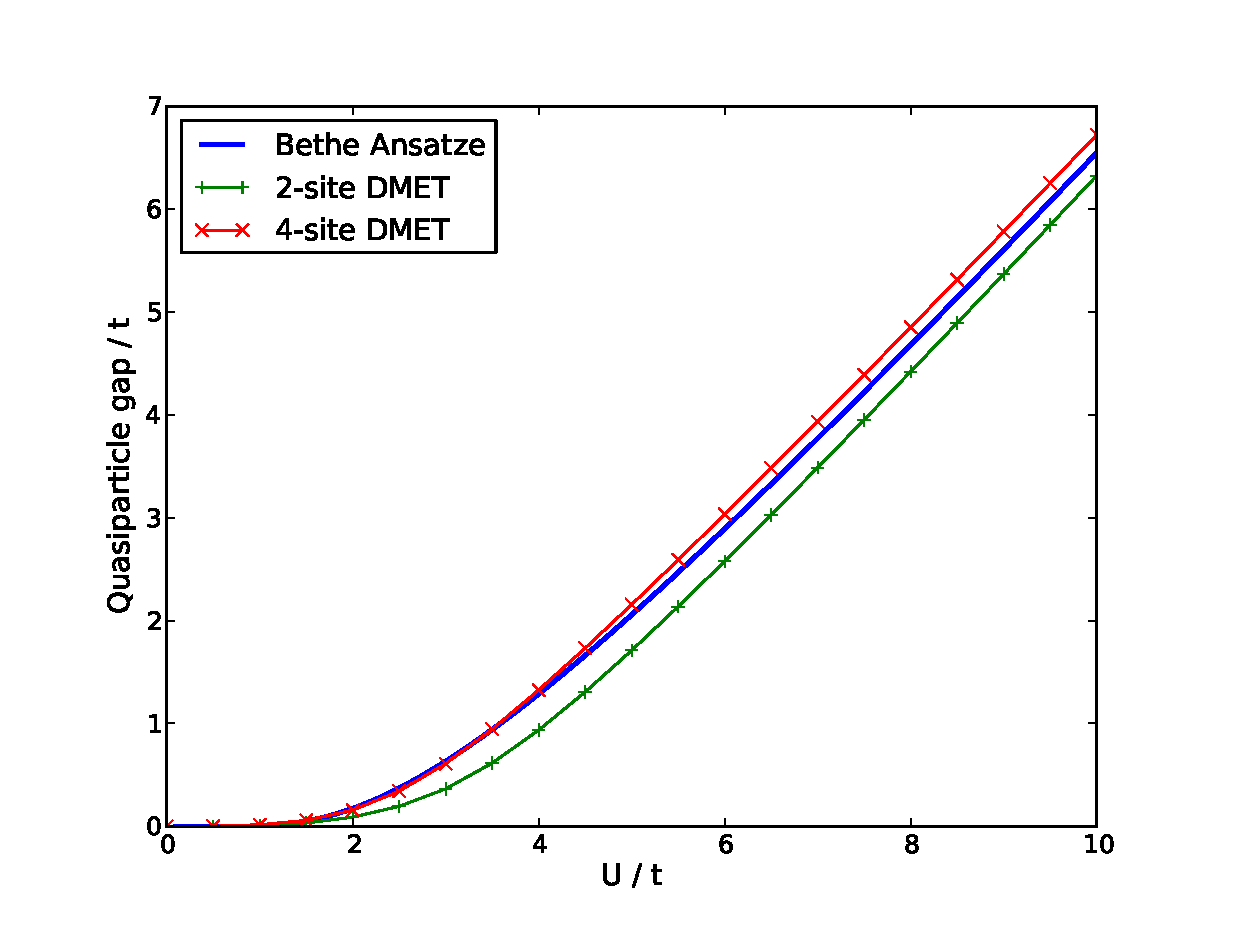
\includegraphics[scale=0.425]{Plots/1D_Gap/Hubbard_Gap.eps}
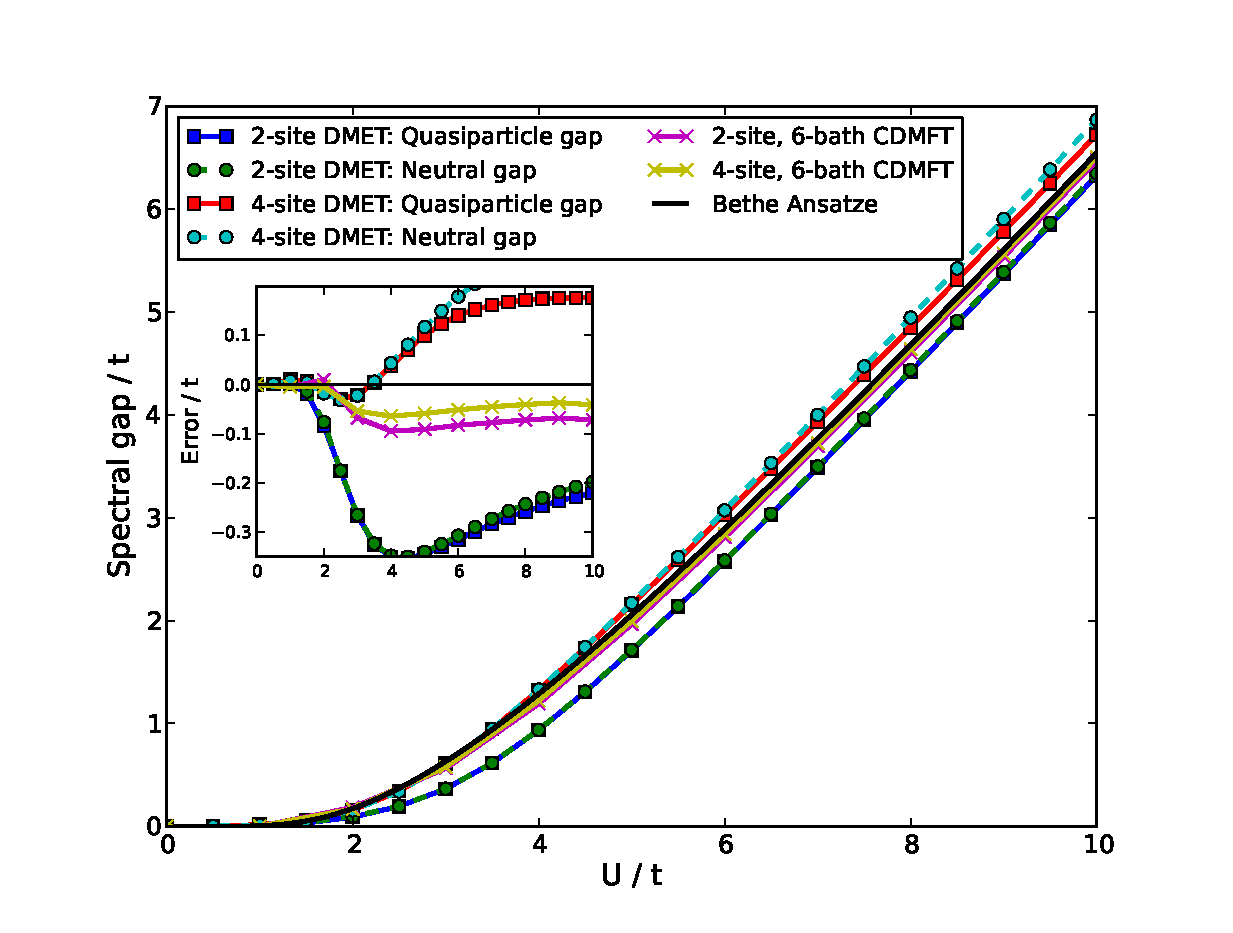
\includegraphics[scale=0.425]{Hubbard_Gap.eps}
\end{center}
    \vspace{-8mm}
\caption{Error in the spectral gap from the impurity 1-particle and 2-particle Green functions compared to analytic results
from the Bethe Ansatze\cite{Ovchinni1970}, and six bath orbital CDMFT+ED lattice Green functions. The results show generally 
good agreement, and convergence of the results with increasing cluster size.}
\label{1D_GAP}
\end{figure}

\emph{Results.-} We first examine the one-dimensional Hubbard model, whose ground state energy\cite{Lieb68} and spectral gap\cite{Ovchinni1970} are 
obtainable from the Bethe Ansatz, and additionally compare to
zero-temperature, cluster DMFT results\cite{Go2009}. Figure~\ref{1D_DOS} shows the local density of states, calculated with a four-site DMET 
impurity cluster, and compared to six-site cluster DMFT results, obtained via an exact diagonalization within six bath orbital representation. 
Both DMET and DMFT calculation are performed in the paramagnetic phase. 
Since exact diagonalization was used as the impurity solver, 
the spectra are obtained on the real axis at zero-temperature, and so can be directly compared against. As expected in the one-dimensional case, there is no
frustration, and the system is dominated at all values of $U$ by long-range magnetic ordering\cite{Lieb68}. Consequently, 
the system is insulating for arbitrarily small values of $U$, in both the DMET and CDMFT spectra. 

The spectral gaps are very similar in the DMET and CDMFT calculations, however, the higher frequency excitations in the CDMFT calculations are very noisy, which makes it difficult to determine 
which features are physical, and which are spurious and a result of the finite (six) bath representation of the coupling of the cluster to the environment. In contrast, the DMET results give an entirely smooth
representation of the spectra, due to the analytic construction of the exact coupling to $|\phi^{(1)}(\omega)\rangle$ at each frequency. However, 
at very high frequencies, outside the bandwidth of $|\phi^{(1)}(\omega)\rangle$, there is no coupling of the local excitations to the 
environment provided by the DMET bath construction and so uncoupled local excitations result. This is related to the frequency 
independence of the local potential $u$, which we have assumed for simplicity as discussed above. 
Therefore, in the results presented, the spectral window probed will be determined by the bandwidth of $|\phi^{(1)}(\omega)\rangle$. Another point to note is that the sum rules on the spectral functions are
exactly obeyed, and the integrated spectral weight of the results in Fig.~\ref{1D_DOS} are all unity.
For comparison, Fig.~\ref{1D_GAP} shows the error in the spectral gap from the exact Bethe Ansatz result\cite{Ovchinni1970}, demonstrating 
the convergence towards the exact spectral gap as the cluster size is increased 
from two to four sites, and indicating a generally similar quality to CDMFT calculations.

%+++++++++++++++++++++++++++++++++++++++++++++++++++++++
%   2D HUBBARD PLOTS 
%+++++++++++++++++++++++++++++++++++++++++++++++++++++++
\begin{figure}
\begin{center}
    \vspace{-2mm}
%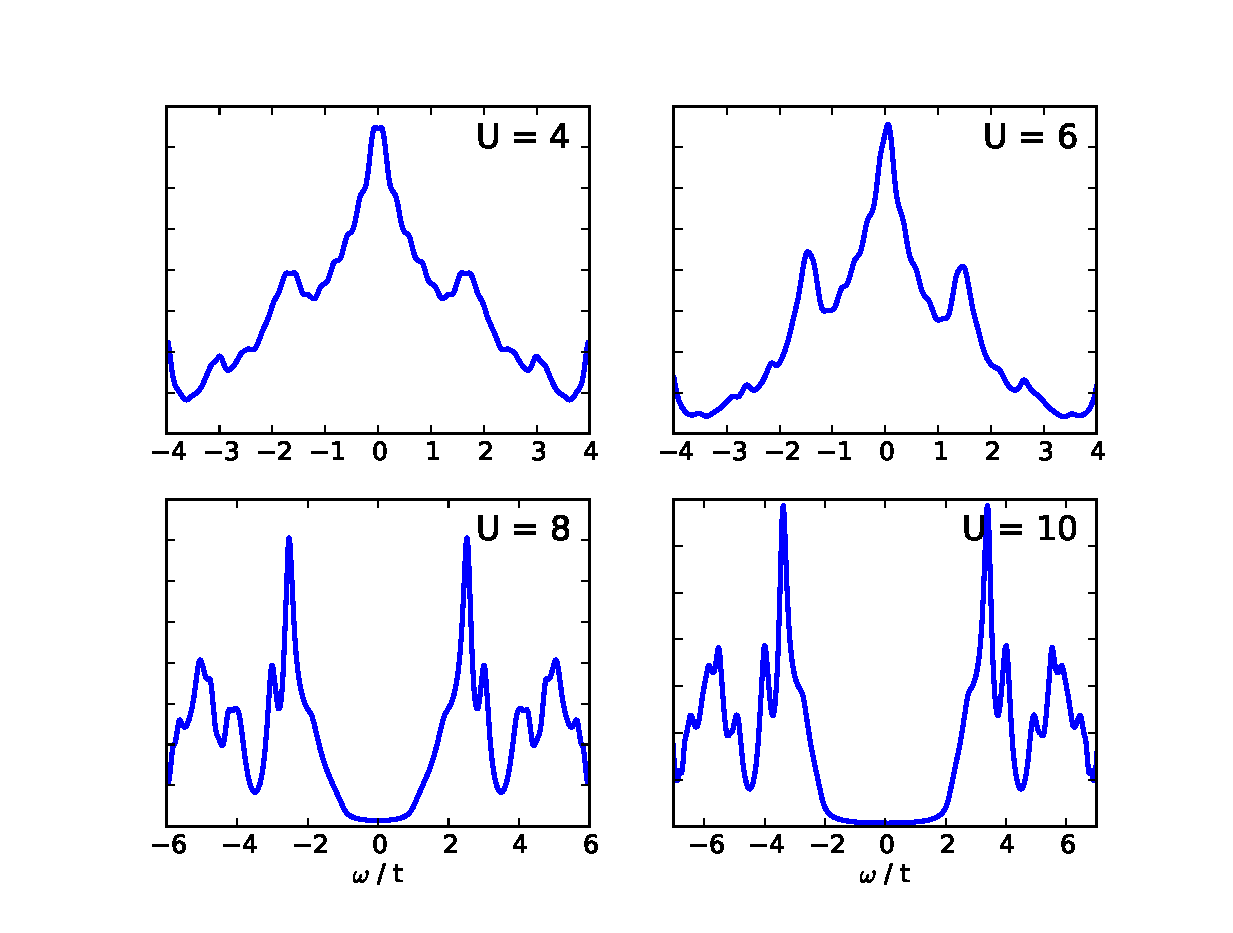
\includegraphics[scale=0.425]{Plots/2D_Spectra/2DHub_Spectra.eps}
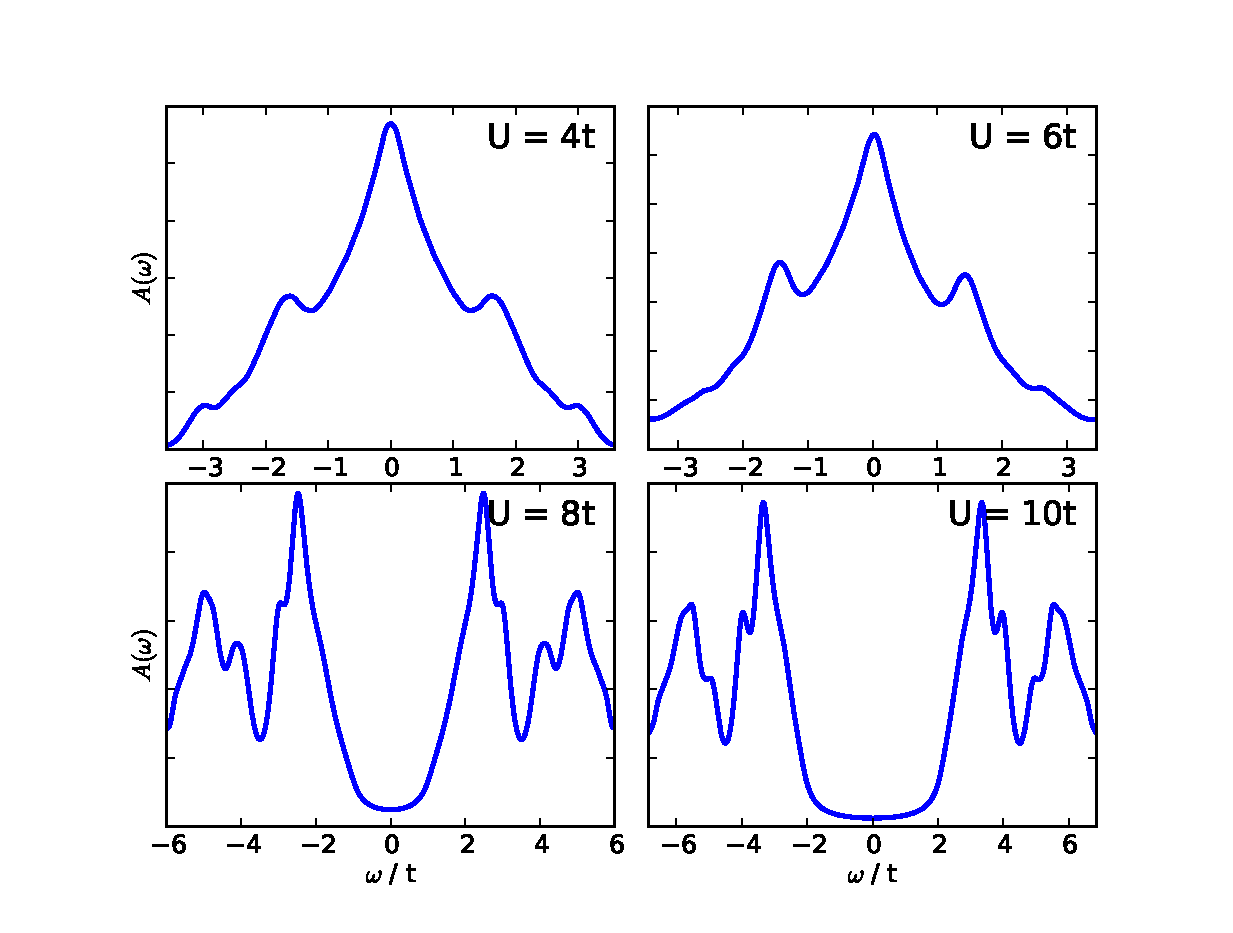
\includegraphics[scale=0.425]{2DHub_Spectra.eps}
\end{center}
    \vspace{-8mm}
\caption{Local density of states of the half-filled 2D Hubbard model from a $2 \times 2$ impurity cluster DMET calculation, with a 
MIT at $U\approx6.9t$. 
The exact bath states from $|\phi^{(1)}(\omega)\rangle$ for each frequency allows for smooth spectral functions at real frequencies.}
%with minimal broadening ($\eta = 0.2t$).}
\label{2D_DOS}
\end{figure}


%+++++++++++++++++++++++++++++++++++++++++++++++++++++++
%   2D DOPED HUBBARD PLOTS 
%+++++++++++++++++++++++++++++++++++++++++++++++++++++++
\begin{figure}
\begin{center}
    \vspace{-2mm}
%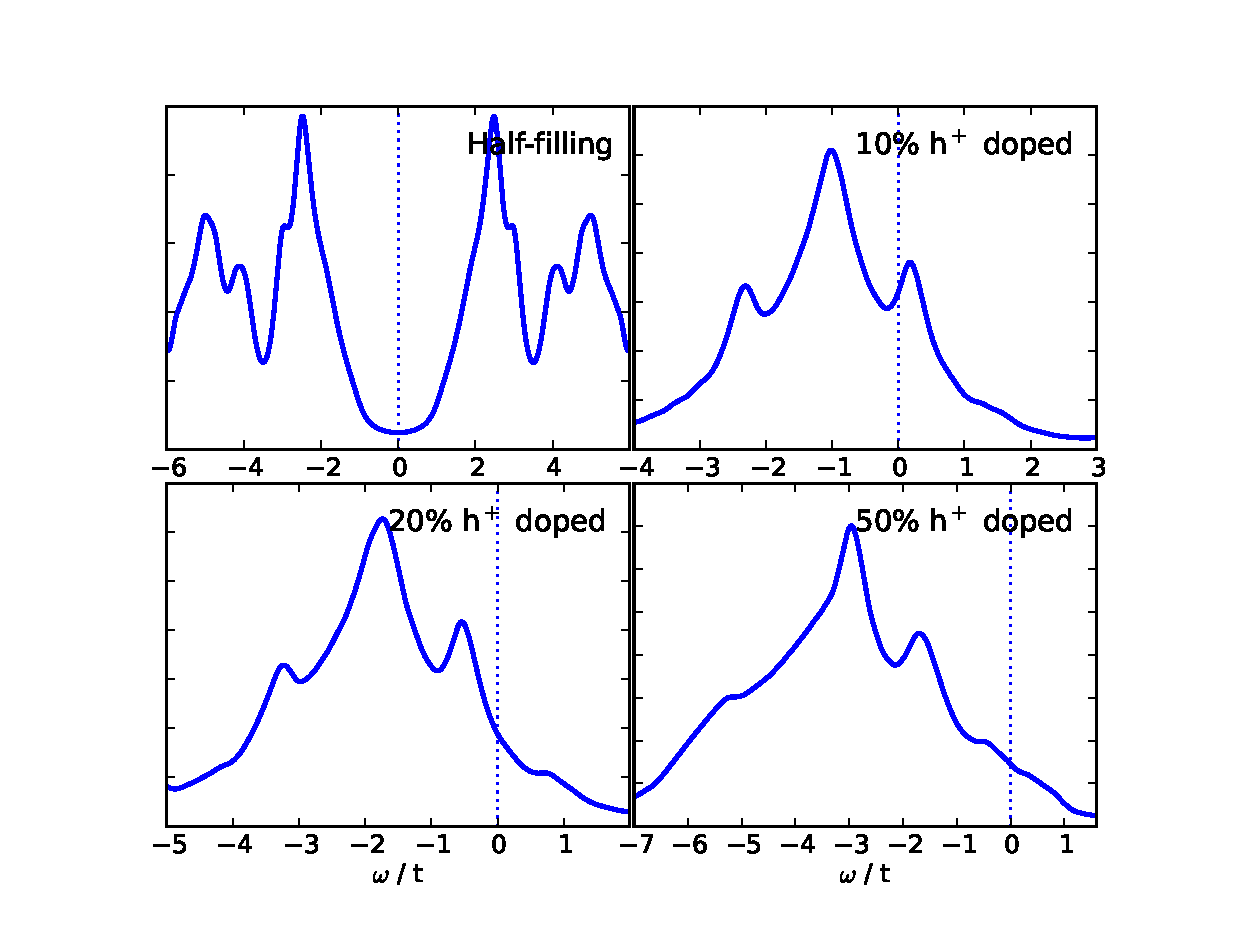
\includegraphics[scale=0.425]{Plots/Doping/2D/nImp4/U8/LargerBroadening/2DHub_Doping.eps}
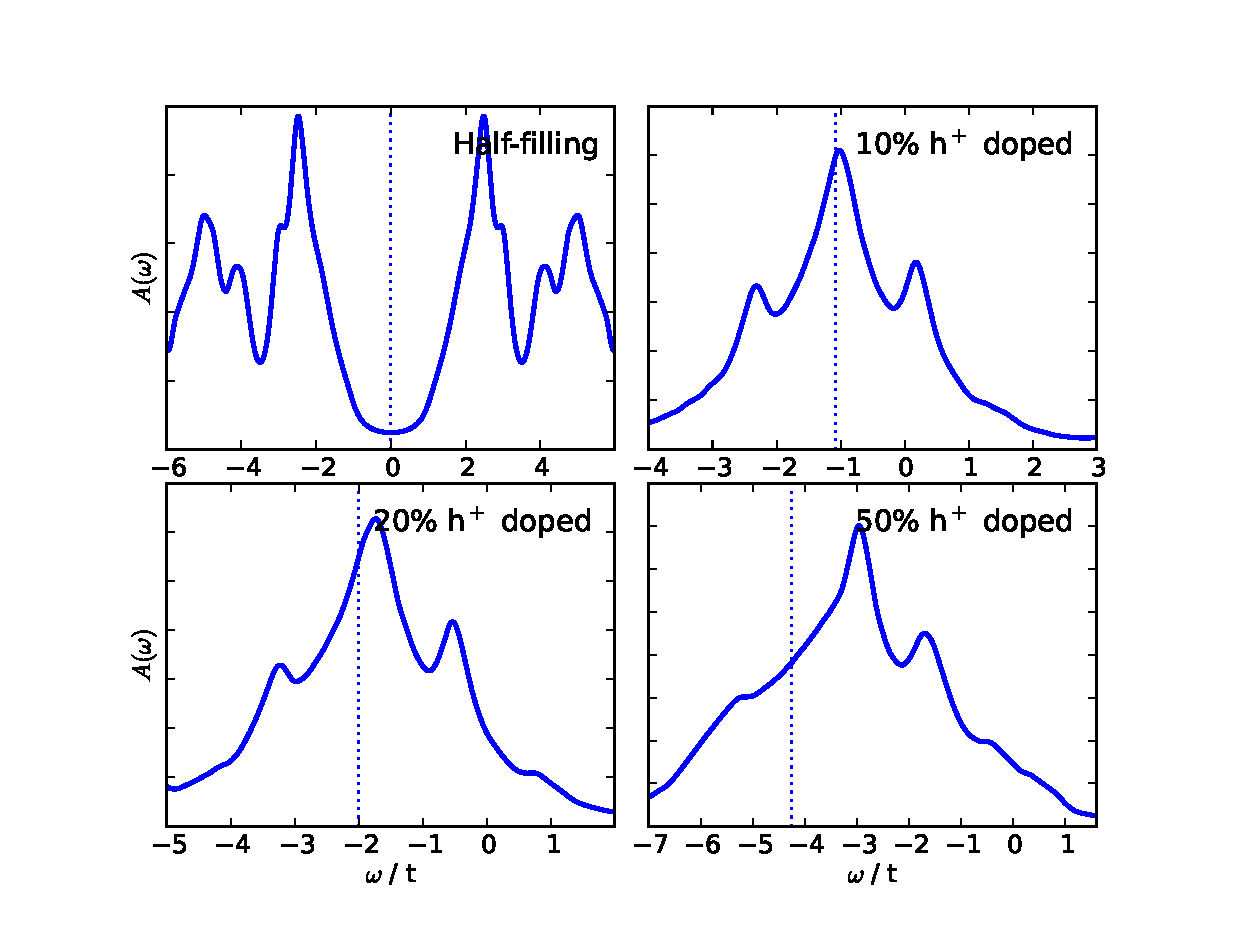
\includegraphics[scale=0.425]{2DHub_Doping.eps}
\end{center}
    \vspace{-8mm}
\caption{Local density of states of the hole doped 2D Hubbard model calculated with a $2 \times 2$ impurity cluster with $U = 8t$. Dotted
lines indicate the Fermi level. Qualitative features present in the CDMFT study of Ref.~\onlinecite{Masatoshi2009} are observed (see Fig. 1(c) and (d)).}
%Aside: Also look at A. Liebsch DMFT in doped Hubbard.}
\label{2D_Doped}
\end{figure}

A sterner test comes from the 2D Hubbard model. Cluster DMFT calculations in the paramagnetic phase exhibit a metal-insulator transition (MIT)
at finite $U$, representative of a Mott transition\cite{Georges1996,Senechal2000,Kotliar2008,Millis2012,Millis2013,Zgid2012}.
%which still receives widespread attention in the condensed matter community\cite{Georges1996,Senechal2000,Kotliar2008,Millis2012,Millis2013}
%due to its first-order metal-insulator transition (MIT) arising from competing magnetic effects as the correlation strength, $U$, is increased. 
The DMET local density of
states are shown in Fig.~\ref{2D_DOS} for a $2 \times 2$ plaquette of impurity sites. In the low $U$ regime, the famous `three-peak' structure 
is observed, with a central Kondo resonance peak, and the Hubbard bands either side. At $U \approx 6.9t$, there is a transition to an insulating 
regime, with a Mott gap opening with increased $U$. The spectra then feature prominent coherence peaks at the gap edge, as have been observed 
elsewhere\cite{Kotliar2008}. Cluster DMFT calculations with the same plaquette size observe a MIT at a slightly lower $U\approx5.5t$, 
with a coexistence region at low temperatures, which we also observe. However, analytically continued
spectral functions from CT-QMC smooth out many of the subtle correlation driven substructures observed in Fig.~\ref{2D_DOS}. 
Fig.~\ref{2D_Doped} shows the effect on the 
spectra upon hole doping the system, which is shown for the insulating phase at $U=8t$. Once doped, the weight is transferred to lower frequencies
until the system becomes a Fermi liquid phase. The spectra are qualitatively similar to those seen in recent cluster DMFT studies\cite{Masatoshi2009}.

%+++++++++++++++++++++++++++++++++++++++++++++++++++++++
%   DD response 
%+++++++++++++++++++++++++++++++++++++++++++++++++++++++
\begin{figure}
\begin{center}
    \vspace{-2mm}
%\includegraphics[scale=0.425]{Plots/2D_DD/2D_DD_Spectra.eps}
\includegraphics[scale=0.425]{2D_DD_Spectra.eps}
\end{center}
    \vspace{-8mm}
\caption{$2 \times 2$ impurity DMET calculation of the local density-density response function for the half-filled 2D Hubbard model.}
\label{2D_DD}
\end{figure}


Fig.~\ref{2D_DD} shows the local density-density response function of the 2D Hubbard model at half-filling, obtained from the local two-particle Green 
function (${\hat V}={\hat X}=\sum_{\sigma} a_{\alpha_{\sigma}}^{\dagger}a_{\alpha_{\sigma}}$). The poles of this 
function correspond to the neutral excitation energies, and as such determine 
the optical properties of the system\cite{Millis2012,Essler91}.
Unfortunately, direct comparison of the spectra in Fig.~\ref{2D_DD} to other results is difficult due to the paucity of other comparable 
calculations for this quantity, but show the expected MIT, and transfer of spectral weight to higher frequencies as $U$ increases.
However, since holons and doublons do not bind in the 1D Hubbard Hamiltonian, 
%exciton binding is negligable, and 
the optical and single-particle gaps obtained should be the same, and these can be tested against the exact Bethe Ansatz results as before\cite{Essler91}. Therefore, excitation gaps
obtained from the two-particle Green functions in the 1D model are included in Fig.~\ref{1D_GAP}, and show that for the same cluster size, the differences between the spectral gaps are generally small.
While not conclusive, this supports the assertion that the one- and two-particle Green functions are of similar quality, while also of comparable computational cost, and validating the results shown in Fig.~\ref{2D_DD}.

In conclusion, we have presented a quantum embedding formalism for accurate, zero-temperature spectral functions of extended, strongly correlated systems 
at a small computational cost, which vastly 
extends the scope of the DMET method. The approach has a number of 
advantageous formal properties. 
\begin{inparaenum}[\itshape i\upshape)]
\item The embedding within the environment is achieved via coupling to a small set of analytically constructed, many-particle bath states,
    which are derived from the formal Schmidt decomposition of the response vector obtained from a one-particle Hamiltonian. The quantum impurity
    plus bath space therefore exactly spans this vector, and
    changes with frequency, to give smooth spectra without any error from the discretization of the continuum.
\item The simple finite size quantum impurity model allows spectral functions to be easily obtained on the real frequency axis, removing the 
    need for any analytic continuation from the imaginary axis.
\item The interacting quantum impurity and bath space is independent of the size of the underlying lattice, and is constructed at a cost no greater than the
    diagonalization of the one-particle Hamiltonian
\item Both extension to clusters of impurity sites, and arbitrary dynamic correlation functions are straightforward within the framework.
\end{inparaenum}
The approach was demonstrated on the one- and two-dimensional Hubbard model, and compared favorably to both exact results and cluster DMFT calculations. Extensions are now underway for the
calculation of non-local operators, an {\em ab initio} formulation, and for the investigation of differently ordered phases by embedding within broken symmetry mean-field Hamiltonians.
%\vskip 5mm 

{\bf Acknowledgements}

The authors would like to sincerely thank Ara Go for sharing unpublished CDMFT results and useful 
conversations, and Cedric Weber and Qiaoni Chen for useful comments on the manuscript.
This work was supported by the DoE through grants DE-SC0010530, and DE-FG02-12ER46875.

%\bibliography{SpectralDMETBib}
\begin{thebibliography}{25}
\expandafter\ifx\csname natexlab\endcsname\relax\def\natexlab#1{#1}\fi
\expandafter\ifx\csname bibnamefont\endcsname\relax
  \def\bibnamefont#1{#1}\fi
\expandafter\ifx\csname bibfnamefont\endcsname\relax
  \def\bibfnamefont#1{#1}\fi
\expandafter\ifx\csname citenamefont\endcsname\relax
  \def\citenamefont#1{#1}\fi
\expandafter\ifx\csname url\endcsname\relax
  \def\url#1{\texttt{#1}}\fi
\expandafter\ifx\csname urlprefix\endcsname\relax\def\urlprefix{URL }\fi
\providecommand{\bibinfo}[2]{#2}
\providecommand{\eprint}[2][]{\url{#2}}

\bibitem[{\citenamefont{Coulter et~al.}(2013)\citenamefont{Coulter, Manousakis,
  and Gali}}]{Gali2013}
\bibinfo{author}{\bibfnamefont{J.~E.} \bibnamefont{Coulter}},
  \bibinfo{author}{\bibfnamefont{E.}~\bibnamefont{Manousakis}},
  \bibnamefont{and} \bibinfo{author}{\bibfnamefont{A.}~\bibnamefont{Gali}}
  (\bibinfo{year}{2013}), \bibinfo{note}{arXiv:1306.4948}.

\bibitem[{\citenamefont{Mukherjee et~al.}(2013)\citenamefont{Mukherjee,
  Sawatzky, and Berciu}}]{Mona2013}
\bibinfo{author}{\bibfnamefont{A.}~\bibnamefont{Mukherjee}},
  \bibinfo{author}{\bibfnamefont{G.~A.} \bibnamefont{Sawatzky}},
  \bibnamefont{and} \bibinfo{author}{\bibfnamefont{M.}~\bibnamefont{Berciu}},
  \bibinfo{journal}{Phys. Rev. B} \textbf{\bibinfo{volume}{87}},
  \bibinfo{pages}{165136} (\bibinfo{year}{2013}).

\bibitem[{\citenamefont{Lin et~al.}(2012)\citenamefont{Lin, Gull, and
  Millis}}]{Millis2012}
\bibinfo{author}{\bibfnamefont{N.}~\bibnamefont{Lin}},
  \bibinfo{author}{\bibfnamefont{E.}~\bibnamefont{Gull}}, \bibnamefont{and}
  \bibinfo{author}{\bibfnamefont{A.~J.} \bibnamefont{Millis}},
  \bibinfo{journal}{Phys. Rev. Lett.} \textbf{\bibinfo{volume}{109}},
  \bibinfo{pages}{106401} (\bibinfo{year}{2012}).

\bibitem[{\citenamefont{Sordi et~al.}(2012)\citenamefont{Sordi, S\'emon, Haule,
  and Tremblay}}]{Sordi2012}
\bibinfo{author}{\bibfnamefont{G.}~\bibnamefont{Sordi}},
  \bibinfo{author}{\bibfnamefont{P.}~\bibnamefont{S\'emon}},
  \bibinfo{author}{\bibfnamefont{K.}~\bibnamefont{Haule}}, \bibnamefont{and}
  \bibinfo{author}{\bibfnamefont{A.-M.~S.} \bibnamefont{Tremblay}},
  \bibinfo{journal}{Phys. Rev. Lett.} \textbf{\bibinfo{volume}{108}},
  \bibinfo{pages}{216401} (\bibinfo{year}{2012}).

\bibitem[{\citenamefont{Gull et~al.}(2013)\citenamefont{Gull, Parcollet, and
  Millis}}]{Millis2013}
\bibinfo{author}{\bibfnamefont{E.}~\bibnamefont{Gull}},
  \bibinfo{author}{\bibfnamefont{O.}~\bibnamefont{Parcollet}},
  \bibnamefont{and} \bibinfo{author}{\bibfnamefont{A.~J.}
  \bibnamefont{Millis}}, \bibinfo{journal}{Phys. Rev. Lett.}
  \textbf{\bibinfo{volume}{110}}, \bibinfo{pages}{216405}
  (\bibinfo{year}{2013}).

\bibitem[{\citenamefont{Georges and Krauth}(1992)}]{Georges1992}
\bibinfo{author}{\bibfnamefont{A.}~\bibnamefont{Georges}} \bibnamefont{and}
  \bibinfo{author}{\bibfnamefont{W.}~\bibnamefont{Krauth}},
  \bibinfo{journal}{Phys. Rev. Lett.} \textbf{\bibinfo{volume}{69}},
  \bibinfo{pages}{1240} (\bibinfo{year}{1992}).

\bibitem[{\citenamefont{Georges et~al.}(1996)\citenamefont{Georges, Kotliar,
  Krauth, and Rozenberg}}]{Georges1996}
\bibinfo{author}{\bibfnamefont{A.}~\bibnamefont{Georges}},
  \bibinfo{author}{\bibfnamefont{G.}~\bibnamefont{Kotliar}},
  \bibinfo{author}{\bibfnamefont{W.}~\bibnamefont{Krauth}}, \bibnamefont{and}
  \bibinfo{author}{\bibfnamefont{M.}~\bibnamefont{Rozenberg}},
  \bibinfo{journal}{Rev. Mod. Phys.} \textbf{\bibinfo{volume}{68}},
  \bibinfo{pages}{13} (\bibinfo{year}{1996}).

\bibitem[{\citenamefont{Kotliar et~al.}(2006)\citenamefont{Kotliar, Savrasov,
  Haule, Oudovenko, Parcollet, and Marianetti}}]{Kotliar2006}
\bibinfo{author}{\bibfnamefont{G.}~\bibnamefont{Kotliar}},
  \bibinfo{author}{\bibfnamefont{S.~Y.} \bibnamefont{Savrasov}},
  \bibinfo{author}{\bibfnamefont{K.}~\bibnamefont{Haule}},
  \bibinfo{author}{\bibfnamefont{V.~S.} \bibnamefont{Oudovenko}},
  \bibinfo{author}{\bibfnamefont{O.}~\bibnamefont{Parcollet}},
  \bibnamefont{and} \bibinfo{author}{\bibfnamefont{C.~A.}
  \bibnamefont{Marianetti}}, \bibinfo{journal}{Rev. Mod. Phys.}
  \textbf{\bibinfo{volume}{78}}, \bibinfo{pages}{865} (\bibinfo{year}{2006}).

\bibitem[{\citenamefont{Werner et~al.}(2006)\citenamefont{Werner, Comanac, de'
  Medici, Troyer, and Millis}}]{Millis2006}
\bibinfo{author}{\bibfnamefont{P.}~\bibnamefont{Werner}},
  \bibinfo{author}{\bibfnamefont{A.}~\bibnamefont{Comanac}},
  \bibinfo{author}{\bibfnamefont{L.}~\bibnamefont{de' Medici}},
  \bibinfo{author}{\bibfnamefont{M.}~\bibnamefont{Troyer}}, \bibnamefont{and}
  \bibinfo{author}{\bibfnamefont{A.~J.} \bibnamefont{Millis}},
  \bibinfo{journal}{Phys. Rev. Lett.} \textbf{\bibinfo{volume}{97}},
  \bibinfo{pages}{076405} (\bibinfo{year}{2006}).

\bibitem[{\citenamefont{Zgid et~al.}(2012)\citenamefont{Zgid, Gull, and
  Chan}}]{Zgid2012}
\bibinfo{author}{\bibfnamefont{D.}~\bibnamefont{Zgid}},
  \bibinfo{author}{\bibfnamefont{E.}~\bibnamefont{Gull}}, \bibnamefont{and}
  \bibinfo{author}{\bibfnamefont{G.~K.-L.} \bibnamefont{Chan}},
  \bibinfo{journal}{Phys. Rev. B} \textbf{\bibinfo{volume}{86}},
  \bibinfo{pages}{165128} (\bibinfo{year}{2012}).

\bibitem[{\citenamefont{Wang et~al.}(2009)\citenamefont{Wang, Gull, de' Medici,
  Capone, and Millis}}]{Millis2009}
\bibinfo{author}{\bibfnamefont{X.}~\bibnamefont{Wang}},
  \bibinfo{author}{\bibfnamefont{E.}~\bibnamefont{Gull}},
  \bibinfo{author}{\bibfnamefont{L.}~\bibnamefont{de' Medici}},
  \bibinfo{author}{\bibfnamefont{M.}~\bibnamefont{Capone}}, \bibnamefont{and}
  \bibinfo{author}{\bibfnamefont{A.}~\bibnamefont{Millis}},
  \bibinfo{journal}{Phys. Rev. B} \textbf{\bibinfo{volume}{80}},
  \bibinfo{pages}{045101} (\bibinfo{year}{2009}).

\bibitem[{\citenamefont{Liebsch and Ishida}(2012)}]{Liebsch2012}
\bibinfo{author}{\bibfnamefont{A.}~\bibnamefont{Liebsch}} \bibnamefont{and}
  \bibinfo{author}{\bibfnamefont{H.}~\bibnamefont{Ishida}},
  \bibinfo{journal}{J. Phys.: Condens. Matter} \textbf{\bibinfo{volume}{24}},
  \bibinfo{pages}{053201} (\bibinfo{year}{2012}).

\bibitem[{\citenamefont{Benthien et~al.}(2004)\citenamefont{Benthien, Gebhard,
  and Jeckelmann}}]{Jeckelmann2004}
\bibinfo{author}{\bibfnamefont{H.}~\bibnamefont{Benthien}},
  \bibinfo{author}{\bibfnamefont{F.}~\bibnamefont{Gebhard}}, \bibnamefont{and}
  \bibinfo{author}{\bibfnamefont{E.}~\bibnamefont{Jeckelmann}},
  \bibinfo{journal}{Phys. Rev. Lett.} \textbf{\bibinfo{volume}{92}},
  \bibinfo{pages}{256401} (\bibinfo{year}{2004}).

\bibitem[{\citenamefont{Senechal et~al.}(2000)\citenamefont{Senechal, Perez,
  and Pioro-Ladiere}}]{Senechal2000}
\bibinfo{author}{\bibfnamefont{D.}~\bibnamefont{Senechal}},
  \bibinfo{author}{\bibfnamefont{D.}~\bibnamefont{Perez}}, \bibnamefont{and}
  \bibinfo{author}{\bibfnamefont{M.}~\bibnamefont{Pioro-Ladiere}},
  \bibinfo{journal}{Phys. Rev. Lett.} \textbf{\bibinfo{volume}{84}},
  \bibinfo{pages}{522} (\bibinfo{year}{2000}).

\bibitem[{\citenamefont{Knizia and Chan}(2012)}]{Chan2012}
\bibinfo{author}{\bibfnamefont{G.}~\bibnamefont{Knizia}} \bibnamefont{and}
  \bibinfo{author}{\bibfnamefont{G.~K.-L.} \bibnamefont{Chan}},
  \bibinfo{journal}{Phys. Rev. Lett.} \textbf{\bibinfo{volume}{109}},
  \bibinfo{pages}{186404} (\bibinfo{year}{2012}).

\bibitem[{\citenamefont{Knizia and Chan}(2013)}]{Chan2013}
\bibinfo{author}{\bibfnamefont{G.}~\bibnamefont{Knizia}} \bibnamefont{and}
  \bibinfo{author}{\bibfnamefont{G.~K.-L.} \bibnamefont{Chan}},
  \bibinfo{journal}{J. Chem. Theory Comput.} \textbf{\bibinfo{volume}{9}},
  \bibinfo{pages}{1428} (\bibinfo{year}{2013}).

\bibitem[{\citenamefont{Limelette et~al.}(2003)\citenamefont{Limelette,
  Georges, Jerome, Wzietek, Metcalf, and Honig}}]{Limelette2003}
\bibinfo{author}{\bibfnamefont{P.}~\bibnamefont{Limelette}},
  \bibinfo{author}{\bibfnamefont{A.}~\bibnamefont{Georges}},
  \bibinfo{author}{\bibfnamefont{D.}~\bibnamefont{Jerome}},
  \bibinfo{author}{\bibfnamefont{P.}~\bibnamefont{Wzietek}},
  \bibinfo{author}{\bibfnamefont{P.}~\bibnamefont{Metcalf}}, \bibnamefont{and}
  \bibinfo{author}{\bibfnamefont{J.}~\bibnamefont{Honig}},
  \bibinfo{journal}{Science} \textbf{\bibinfo{volume}{302}},
  \bibinfo{pages}{89} (\bibinfo{year}{2003}).

\bibitem[{\citenamefont{Anderson}(1987)}]{Anderson87}
\bibinfo{author}{\bibfnamefont{P.~W.} \bibnamefont{Anderson}},
  \bibinfo{journal}{Science} \textbf{\bibinfo{volume}{235}},
  \bibinfo{pages}{1196} (\bibinfo{year}{1987}).

\bibitem[{\citenamefont{Lieb and Wu}(1968)}]{Lieb68}
\bibinfo{author}{\bibfnamefont{E.}~\bibnamefont{Lieb}} \bibnamefont{and}
  \bibinfo{author}{\bibfnamefont{F.}~\bibnamefont{Wu}}, \bibinfo{journal}{Phys.
  Rev. Lett.} \textbf{\bibinfo{volume}{20}}, \bibinfo{pages}{1445}
  (\bibinfo{year}{1968}).

\bibitem[{\citenamefont{Ovchinni}(1970)}]{Ovchinni1970}
\bibinfo{author}{\bibfnamefont{A.}~\bibnamefont{Ovchinni}},
  \bibinfo{journal}{Sov. Phys. JETP-USSR} \textbf{\bibinfo{volume}{30}},
  \bibinfo{pages}{1160} (\bibinfo{year}{1970}).

\bibitem[{\citenamefont{Go and Jeon}(2009)}]{Go2009}
\bibinfo{author}{\bibfnamefont{A.}~\bibnamefont{Go}} \bibnamefont{and}
  \bibinfo{author}{\bibfnamefont{G.~S.} \bibnamefont{Jeon}},
  \bibinfo{journal}{J. Phys.: Condens. Mat.} \textbf{\bibinfo{volume}{21}},
  \bibinfo{pages}{485602} (\bibinfo{year}{2009}).

\bibitem[{\citenamefont{Park et~al.}(2008)\citenamefont{Park, Haule, and
  Kotliar}}]{Kotliar2008}
\bibinfo{author}{\bibfnamefont{H.}~\bibnamefont{Park}},
  \bibinfo{author}{\bibfnamefont{K.}~\bibnamefont{Haule}}, \bibnamefont{and}
  \bibinfo{author}{\bibfnamefont{G.}~\bibnamefont{Kotliar}},
  \bibinfo{journal}{Phys. Rev. Lett.} \textbf{\bibinfo{volume}{101}},
  \bibinfo{pages}{186403} (\bibinfo{year}{2008}).

\bibitem[{\citenamefont{Sakai et~al.}(2009)\citenamefont{Sakai, Motome, and
  Imada}}]{Masatoshi2009}
\bibinfo{author}{\bibfnamefont{S.}~\bibnamefont{Sakai}},
  \bibinfo{author}{\bibfnamefont{Y.}~\bibnamefont{Motome}}, \bibnamefont{and}
  \bibinfo{author}{\bibfnamefont{M.}~\bibnamefont{Imada}},
  \bibinfo{journal}{Phys. Rev. Lett.} \textbf{\bibinfo{volume}{102}},
  \bibinfo{pages}{056404} (\bibinfo{year}{2009}).

\bibitem[{\citenamefont{Fraysse et~al.}(2005)\citenamefont{Fraysse, Giraud,
  Gratton, and Langou}}]{Langou2005}
\bibinfo{author}{\bibfnamefont{V.}~\bibnamefont{Fraysse}},
  \bibinfo{author}{\bibfnamefont{L.}~\bibnamefont{Giraud}},
  \bibinfo{author}{\bibfnamefont{S.}~\bibnamefont{Gratton}}, \bibnamefont{and}
  \bibinfo{author}{\bibfnamefont{J.}~\bibnamefont{Langou}},
  \bibinfo{journal}{ACM T. Math. Software} \textbf{\bibinfo{volume}{31}},
  \bibinfo{pages}{228} (\bibinfo{year}{2005}).

\bibitem[{\citenamefont{Essler et~al.}(1991)\citenamefont{Essler, Korepin, and
  Schoutens}}]{Essler91}
\bibinfo{author}{\bibfnamefont{F.}~\bibnamefont{Essler}},
  \bibinfo{author}{\bibfnamefont{V.}~\bibnamefont{Korepin}}, \bibnamefont{and}
  \bibinfo{author}{\bibfnamefont{K.}~\bibnamefont{Schoutens}},
  \bibinfo{journal}{Phys. Rev. Lett.} \textbf{\bibinfo{volume}{67}},
  \bibinfo{pages}{3848} (\bibinfo{year}{1991}).

\end{thebibliography}

\end{document}
